\documentclass[a4paper,12pt]{article}

% ==================== 宏包导入 ====================
\usepackage[UTF8, scheme=chinese, heading=true]{ctex}
\usepackage{geometry}
\usepackage{titlesec}
\usepackage{graphicx}
\usepackage{float}
\usepackage{amsmath}
\usepackage{amsfonts}
\usepackage{amssymb}
\usepackage{booktabs}
\usepackage{listings}
\usepackage{xcolor}
\usepackage[hidelinks]{hyperref}
\usepackage{caption}
\usepackage{subcaption}
\usepackage{fancyhdr}
\usepackage{algorithm}
\usepackage{algorithmic}
\usepackage{enumitem}
\usepackage{times} % 英文字体 Times New Roman
\usepackage{setspace}
\usepackage{multirow}
\usepackage{cite}
\usepackage{pdfpages}

% ==================== 绘图支持 (TikZ) ====================
\usepackage{tikz}
\usetikzlibrary{shapes.geometric, arrows}

% 定义流程图样式
\tikzstyle{startstop} = [rectangle, rounded corners, minimum width=3cm, minimum height=1cm,text centered, draw=black, fill=red!30]
\tikzstyle{io} = [trapezium, trapezium left angle=70, trapezium right angle=110, minimum width=3cm, minimum height=1cm, text centered, draw=black, fill=blue!30]
\tikzstyle{process} = [rectangle, minimum width=3cm, minimum height=1cm, text centered, draw=black, fill=orange!30]
\tikzstyle{decision} = [diamond, minimum width=3cm, minimum height=1cm, text centered, draw=black, fill=green!30, aspect=2.5]
\tikzstyle{arrow} = [thick,->,>=stealth]

% ==================== 页面与格式设置 ====================
% 页边距
\geometry{left=2.5cm,right=2.5cm,top=2.5cm,bottom=2.5cm}

% 行距：1.25倍 (Word中的1.5倍视感，适合阅读)
\setstretch{1.25} 

% 正文默认字体：小四号宋体
\renewcommand{\normalsize}{\zihao{-4}\songti}

% 标题格式设置
% 一级标题：三号宋体加粗，左对齐
\titleformat{\section}{\zihao{3}\songti\bfseries\raggedright}{\thesection.}{0.5em}{}
% 二级标题：四号宋体加粗，左对齐
\titleformat{\subsection}{\zihao{4}\songti\bfseries\raggedright}{\thesubsection}{0.5em}{}
% 三级标题：小四号宋体加粗，左对齐
\titleformat{\subsubsection}{\zihao{-4}\songti\bfseries\raggedright}{\thesubsubsection}{0.5em}{}

% 题目页设置
\makeatletter
\renewcommand{\maketitle}{
  \begin{center}
    \vspace*{2em}
    {\zihao{2}\songti\bfseries \@title \par}
    \vspace{2em}
    {\zihao{-4}\songti \@author \par}
    \vspace{1em}
    {\zihao{-4}\songti \@date \par}
    \vspace{3em}
  \end{center}
}
\makeatother

% 页眉页脚
\setlength{\headheight}{15pt}
\pagestyle{fancy}
\fancyhf{}
\fancyhead[C]{\zihao{-5}\songti 嵌入式Linux系统更新机制研究}
\fancyfoot[C]{\zihao{-5}\thepage}

% 代码块样式
\lstset{
    basicstyle=\footnotesize\ttfamily,
    keywordstyle=\color{blue}\bfseries,
    breaklines=true,
    frame=shadowbox,
    numbers=left,
    numberstyle=\tiny,
    captionpos=b,
    tabsize=4
}

% ==================== 论文信息 ====================
\title{嵌入式Linux系统更新机制研究：\\原理、流程与工业级可靠性设计\\——以U-Boot与Mfgtool为例}
\date{2025年12月31日}

% ==================== 正文开始 ====================
\begin{document}

% 封面 (如不需要可注释)
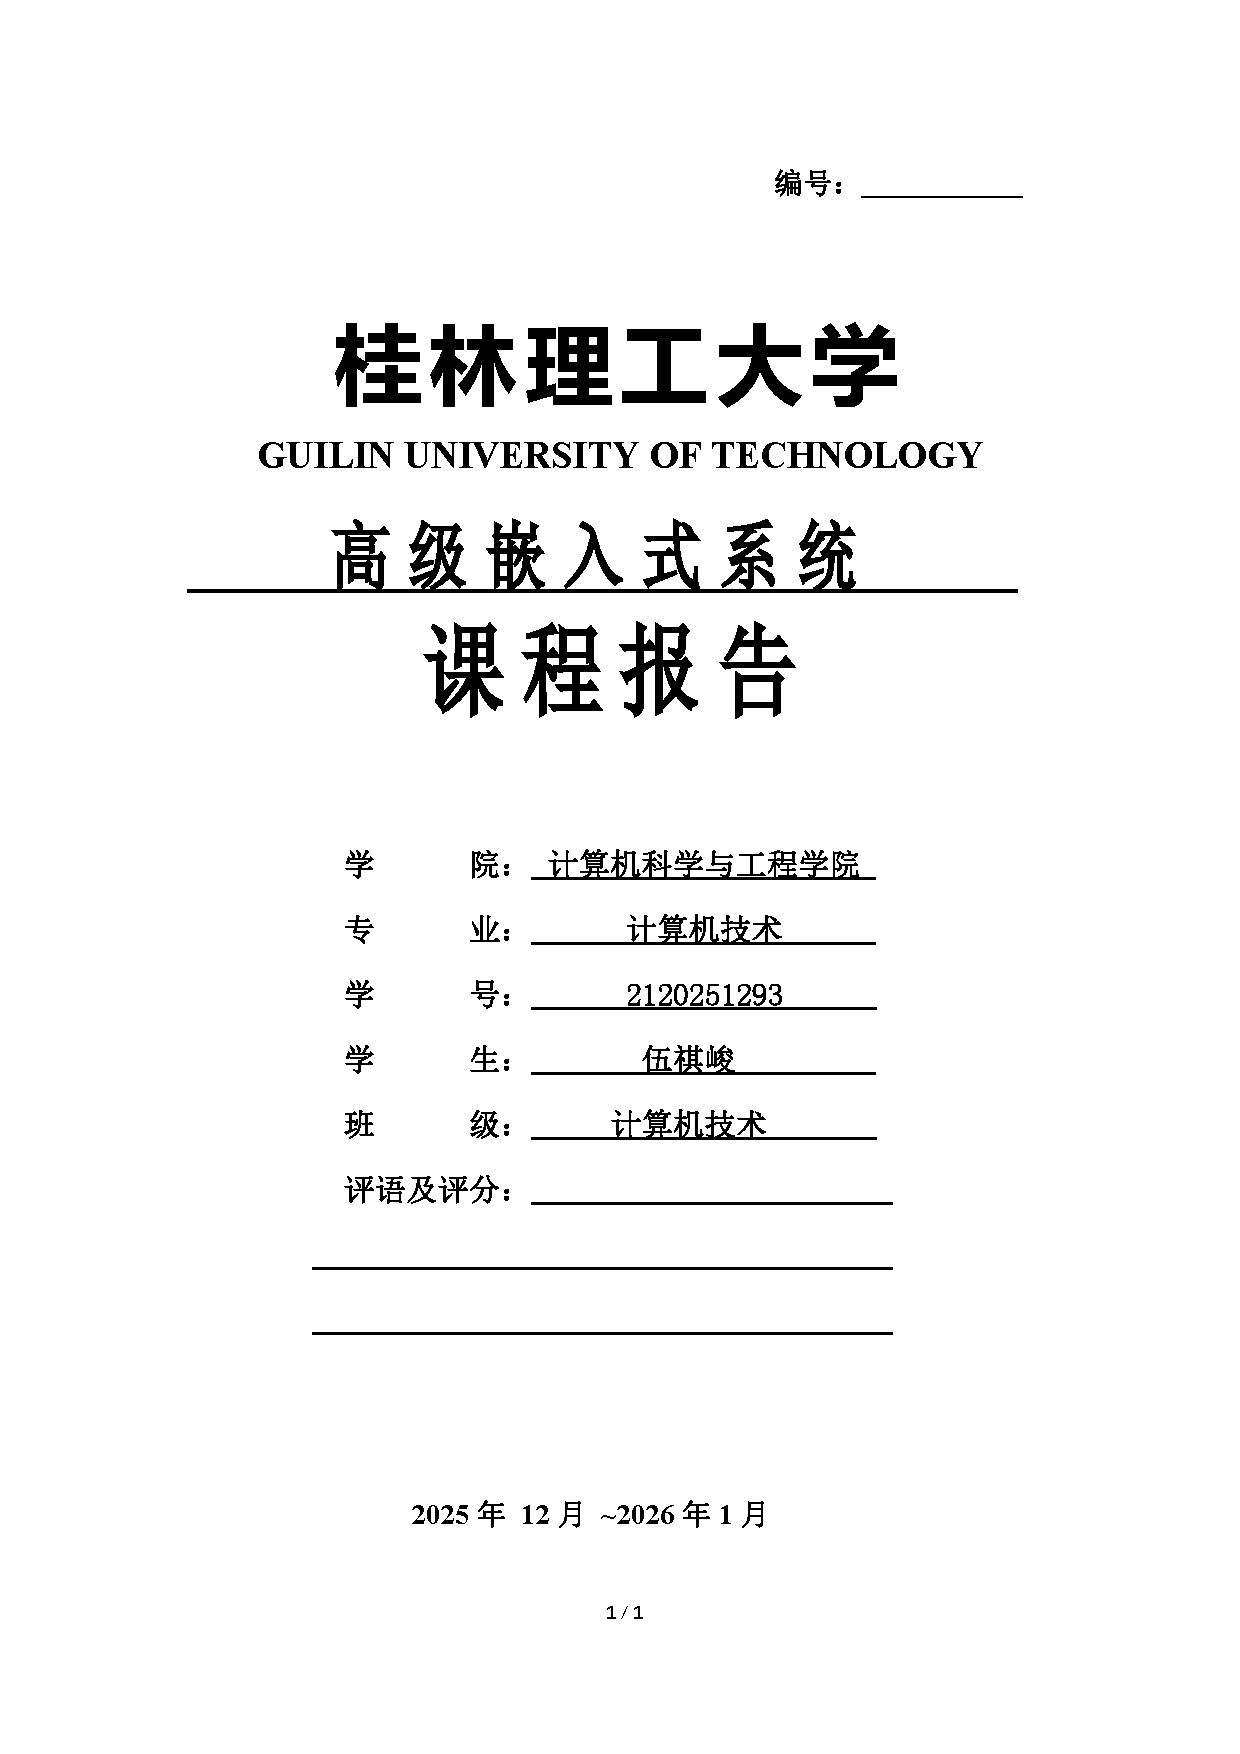
\includepdf[pages=-]{../../covers/ks/高级嵌入式-封面.pdf}

\maketitle

% ==================== 摘要 ====================
\begin{abstract}
\zihao{-4}\songti
\noindent
\textbf{背景:} 随着工业4.0与工业物联网(IIoT)的深入发展，嵌入式设备在复杂环境下的全生命周期管理面临严峻挑战。Mirani等人的研究表明，IIoT架构的异构性和规模化使得边缘设备的维护变得异常复杂，传统的系统更新方法已难以满足现代工业场景的需求\cite{Mirani2022}。

\textbf{目的:} 本文旨在系统深入地分析嵌入式Linux系统中两种主流的更新机制——基于物理介质的SD卡烧写与基于USB OTG协议的Mfgtool在线更新。在此基础上，结合现有学术研究成果，探讨适用于工业场景的高可靠性、高安全性系统更新架构设计方法论。

\textbf{方法:} 首先，深入剖析i.MX6系列处理器的启动引导流程(Boot Flow)及U-Boot在其中的核心作用。其次，从协议层和操作层详细解构SD卡冷启动更新机制与Mfgtool串行下载协议(SDP)的工作原理。通过搭建实验环境，对比不同更新方式在效率与安全性方面的表现。最后，基于Cebel等人提出的平台无关OTA方法\cite{Cebel2022}、Huang等人基于ARM TrustZone的安全更新方案STBEAT\cite{Huang2022}以及Li等人关于BadUSB攻击的研究\cite{Li2025}，构建了一套抗掉电、防篡改的工业级更新架构。

\textbf{结论:} 研究表明，Mfgtool在批量生产效率上具有显著优势，但在开放环境中存在BadUSB攻击风险；传统的SD卡烧写方式简单可靠但效率低下。通过引入A/B双分区冗余机制及硬件信任根（Root of Trust），可以有效解决传统更新方式中的“变砖”风险与安全漏洞，满足工业级系统的高可用性要求。

\vspace{0.5cm}
\noindent \textbf{关键词:} 嵌入式Linux; U-Boot; Mfgtool; OTA更新; 可靠性设计; ARM TrustZone; BadUSB
\end{abstract}

\newpage
\tableofcontents
\newpage

% ==================== 第一章 引言 ====================
\section{引言}

\subsection{研究背景与意义}
嵌入式系统已成为现代工业基础设施的核心组成部分。然而，Mirani等人在其关于工业物联网架构的研究中指出，IIoT系统的异构性(heterogeneity)和规模化(scalability)特征使得边缘设备的生命周期管理变得异常复杂\cite{Mirani2022}。设备不仅需要功能迭代，更需要及时的安全补丁以抵御日益增长的网络威胁。

传统的现场维护方式不仅成本高昂（单次上门成本可达数百元），而且在密封型设备、高危环境（如化工厂、矿井）中难以实施。因此，建立一套安全、可靠、高效的远程更新机制已成为工业界的迫切需求。

\subsection{研究现状与挑战}
在实际工程应用中，系统更新面临三大核心挑战：

\textbf{(1) 可靠性挑战:} 更新过程中的断电可能导致系统无法启动。Marevac等人强调，嵌入式系统必须具备从错误状态自动恢复的能力\cite{Marevac2025}。传统的单分区覆盖式更新一旦中断，会导致启动分区损坏，设备彻底无法启动。

\textbf{(2) 安全性挑战:} Li等人在2025年的研究中揭示了USB接口易受BadUSB攻击的风险\cite{Li2025}。攻击者可通过伪装成HID设备或存储设备的恶意USB硬件，绕过操作系统层的安全检查。而Huang等人则提出了基于ARM TrustZone的防御方案\cite{Huang2022}。

\textbf{(3) 效率挑战:} Shen和Chiang早期的研究指出了完整镜像更新对带宽的巨大消耗\cite{Shen2007}。在低带宽的工业网络环境下，如何减少数据传输量是一个关键问题。

本文将围绕上述挑战，以广泛使用的NXP i.MX6处理器和U-Boot引导加载程序为对象，深入探讨系统更新的原理与优化设计。

% ==================== 第二章 理论基础 ====================
\newpage
\section{嵌入式Linux启动与更新理论基础}

\subsection{ARM SoC启动流程详解}
典型的ARM Cortex-A系列处理器（如NXP i.MX6系列）启动流程包含四个关键阶段，形成一条完整的信任链(Chain of Trust)。

\begin{figure}[H]
\centering
\begin{tikzpicture}[node distance=2cm]
    \zihao{-5} 
    \node (start) [startstop] {上电复位 (Power On)};
    \node (rom) [process, below of=start] {BootROM (固化代码)};
    \node (spl) [process, below of=rom] {SPL (二级引导)};
    \node (uboot) [process, below of=spl] {U-Boot (主引导)};
    \node (kernel) [process, below of=uboot] {Linux Kernel};
    \node (rootfs) [startstop, below of=kernel] {Root Filesystem};

    \draw [arrow] (start) -- (rom);
    \draw [arrow] (rom) -- node[anchor=west] {读取启动引脚} (spl);
    \draw [arrow] (spl) -- node[anchor=west] {初始化DDR} (uboot);
    \draw [arrow] (uboot) -- node[anchor=west] {加载设备树} (kernel);
    \draw [arrow] (kernel) -- node[anchor=west] {挂载文件系统} (rootfs);
\end{tikzpicture}
\caption{基于i.MX6的嵌入式Linux典型启动流程}
\label{fig:boot_flow}
\end{figure}

\subsubsection{BootROM与SPL阶段}
BootROM是SoC内部的只读存储器。上电后，CPU复位向量指向BootROM。它读取启动配置引脚（Boot Mode Pins）确定启动设备（SD卡、eMMC、USB等），并加载SPL（Secondary Program Loader）。

SPL的主要任务包括初始化DDR内存控制器、设置时钟树以及加载完整的U-Boot镜像到DDR中。由于BootROM内部的SRAM容量极为有限（通常仅64KB至256KB），SPL必须保持精简，仅包含最基本的硬件初始化代码。

\subsubsection{U-Boot阶段}
U-Boot是整个启动流程的核心，也是系统更新逻辑的主要执行者。其关键作用包括：
\begin{itemize}
    \item \textbf{环境变量管理:} 维护 \texttt{bootcmd}, \texttt{bootargs} 等关键变量，这些变量决定了系统的启动路径。
    \item \textbf{启动计数器:} 利用 \texttt{boot\_count} 变量记录启动尝试次数，是实现自动回滚的基础。
    \item \textbf{设备树加载:} 解析设备树二进制(DTB)文件，为Linux内核提供硬件描述信息。
\end{itemize}

\subsection{存储分区策略}
为了实现可靠的更新，必须对存储介质进行合理的分区。传统的单分区策略在更新时需要覆盖当前运行的文件系统，风险极高。

本研究采用A/B双分区冗余布局，借鉴Android系统的Seamless Update机制：
\begin{itemize}
    \item \textbf{Bootloader分区:} 存放U-Boot，通常为只读，更新频率极低。
    \item \textbf{Slot A (Kernel + Rootfs):} 主运行分区。
    \item \textbf{Slot B (Kernel + Rootfs):} 备份/更新分区。
    \item \textbf{Data分区:} 存放用户配置文件和日志，更新时不擦除。
\end{itemize}

% ==================== 第三章 主流更新机制剖析 ====================
\newpage
\section{主流更新机制对比分析}

\subsection{基于SD卡的冷启动烧写}
SD卡烧写利用SoC的启动模式选择机制。用户需通过跳线或拨码开关将 BOOT\_MODE 设置为 SD 卡启动。BootROM检测到SD卡后，从预定义的偏移地址加载U-Boot镜像。

\textbf{适用性分析:}
\begin{itemize}
    \item \textbf{优点:} 物理隔离，不依赖网络，适合研发调试和小批量生产。
    \item \textbf{缺点:} 效率低下，Shen和Chiang指出，物理介质插拔难以满足大规模部署需求\cite{Shen2007}。此外，SD卡接触不良增加了故障率。
\end{itemize}

\subsection{基于Mfgtool的USB OTG在线更新}

\subsubsection{技术原理}
Mfgtool基于NXP的SDP（Serial Download Protocol）协议。当设备通过USB OTG连接PC并进入特定模式时，BootROM枚举为HID设备，接收主机指令。

\begin{figure}[H]
\centering
\begin{tikzpicture}[node distance=1.8cm]
    \zihao{-5}
    \node (pc) [startstop, fill=gray!20] {PC端 (Mfgtool)};
    \node (dev) [startstop, fill=gray!20, right of=pc, xshift=5cm] {设备端 (i.MX6)};
    
    \node (step1) [process, below of=pc, yshift=-0.5cm] {1. 识别VID/PID (USB HID)};
    \node (step2) [io, below of=step1] {2. 下发 U-Boot.imx};
    \node (step3) [process, below of=step2] {3. 跳转执行 (Jump)};
    \node (step4) [io, below of=step3] {4. 下发 Kernel \& Ramdisk};
    \node (step5) [process, below of=step4] {5. 启动临时Linux系统};
    \node (step6) [process, below of=step5] {6. 执行烧写脚本 (dd命令)};

    \draw [arrow] (step1) -- (step2);
    \draw [arrow] (step2) -- (step3);
    \draw [arrow] (step3) -- (step4);
    \draw [arrow] (step4) -- (step5);
    \draw [arrow] (step5) -- (step6);
    
    \draw [dashed, ->] (pc) -- node[above]{USB连接} (dev);
\end{tikzpicture}
\caption{Mfgtool基于SDP协议的交互烧写流程}
\label{fig:mfgtool_flow}
\end{figure}

\subsubsection{安全性风险}
虽然Mfgtool效率极高，但Li等人在ByteBait USB的研究中指出，USB接口的物理可访问性使其成为重要攻击面\cite{Li2025}。恶意的USB设备可能模拟Mfgtool的握手过程，尝试注入恶意固件。如果未启用安全启动（Secure Boot），攻击者可轻易通过SDP协议加载未签名的引导程序，获取系统控制权。

\subsection{基于网络的OTA更新}
Cebel等人提出的平台无关OTA方法强调了协议选择的灵活性\cite{Cebel2022}。在工业环境中，考虑到网络的不稳定性，Shen和Chiang建议采用增量更新（差分更新）技术\cite{Shen2007}。

OTA更新的核心在于原子性：下载、校验、写入、切换必须作为一个整体事务。任何环节失败，系统都应保持原状态不变。

% ==================== 第四章 工业级可靠性设计 ====================
\newpage
\section{工业级高可靠性系统更新设计}

\subsection{A/B双分区与自动回滚}
为了解决断电导致的系统损坏问题，本文设计了基于状态机的自动回滚机制。该机制利用U-Boot的环境变量 \texttt{boot\_count} 和 \texttt{boot\_limit} 来监控启动稳定性。

\begin{algorithm}[H]
\caption{双分区自动回滚逻辑}
\begin{algorithmic}[1]
\STATE U-Boot读取 \texttt{boot\_count}
\IF{$\texttt{boot\_count} > \texttt{BOOT\_LIMIT}$}
    \STATE 检测到多次启动失败，执行回滚
    \STATE 切换 \texttt{boot\_part} 指向旧分区
    \STATE 重置 \texttt{boot\_count} = 0
    \STATE 保存环境变量并重启
\ELSE
    \STATE \texttt{boot\_count}++
    \STATE 保存环境变量
    \STATE 尝试从当前 \texttt{boot\_part} 启动内核
\ENDIF
\end{algorithmic}
\end{algorithm}

\begin{figure}[H]
\centering
\begin{tikzpicture}[node distance=2.5cm]
    \zihao{-5}
    \node (start) [startstop] {U-Boot启动};
    \node (read) [process, below of=start, yshift=0.5cm] {读取 boot\_count};
    \node (decide) [decision, below of=read] {boot\_count > Limit?};
    
    \node (normal) [process, left of=decide, xshift=-2.5cm] {boot\_count ++};
    \node (save1) [process, below of=normal, yshift=0.5cm] {保存环境变量};
    \node (bootA) [startstop, below of=save1, yshift=0.5cm] {启动当前分区 (Try)};
    
    \node (rollback) [process, right of=decide, xshift=2.5cm] {执行回滚策略};
    \node (switch) [process, below of=rollback, yshift=0.5cm] {切换 boot\_part};
    \node (reset) [process, below of=switch, yshift=0.5cm] {重置 boot\_count = 0};
    \node (bootB) [startstop, below of=reset, yshift=0.5cm] {启动旧分区 (Stable)};

    \draw [arrow] (start) -- (read);
    \draw [arrow] (read) -- (decide);
    
    \draw [arrow] (decide) -- node[anchor=south] {否 (正常)} (normal);
    \draw [arrow] (normal) -- (save1);
    \draw [arrow] (save1) -- (bootA);
    
    \draw [arrow] (decide) -- node[anchor=south] {是 (异常)} (rollback);
    \draw [arrow] (rollback) -- (switch);
    \draw [arrow] (switch) -- (reset);
    \draw [arrow] (reset) -- (bootB);
\end{tikzpicture}
\caption{A/B分区自动回滚判定逻辑图}
\label{fig:rollback_logic}
\end{figure}

\subsection{基于TrustZone的安全启动}
Huang等人在STBEAT方案中阐述了利用ARM TrustZone保护更新过程的方法\cite{Huang2022}。TrustZone将系统划分为普通世界（Normal World）和安全世界（Secure World）。

在更新场景中，签名验证服务运行在Secure World中。Normal World下载更新包后，必须通过SMC指令请求Secure World进行签名验证。公钥哈希存储在一次性可编程熔丝（OTP）中，确保即使操作系统内核被攻破，攻击者也无法伪造合法的固件签名。

% ==================== 第五章 实验综述与分析 ====================
\newpage
\section{实验综述与分析}

本章基于现有文献中的实验数据与测试模型，对不同的嵌入式Linux更新机制进行综合评估。

\subsection{更新效率与资源消耗对比}
Nagesh等人在其关于BSP现场升级的研究中，对比了不同烧写方式的时间成本。实验表明，在批量部署阶段，并行化的USB烧写（类似Mfgtool机制）比传统的SD卡冷启动方式具有显著的效率优势\cite{Nagesh2019}。

此外，Shen和Chiang的研究量化了全量更新与差分更新的带宽消耗。在低带宽网络环境下，基于差分的机制可以大幅减少数据传输量\cite{Shen2007}。

\begin{table}[H]
\centering
\caption{不同更新机制的效率评估（基于文献数据综述）}
\begin{tabular}{p{3cm}p{3cm}p{4cm}p{3cm}}
\toprule
\textbf{更新方式} & \textbf{主要瓶颈} & \textbf{典型耗时特征} & \textbf{数据来源} \\
\midrule
SD卡冷启动 & 人工插拔、I/O & 高（受限于物理操作） & Nagesh (2019) \\
Mfgtool (USB) & USB总线带宽 & 低（适合并行批量处理） & 厂商技术文档 \\
全量网络OTA & 网络带宽 & 高（随镜像大小线性增长） & Shen (2007) \\
差分/增量OTA & 计算资源 & \textbf{极低} (仅传输差异部分) & Shen (2007) \\
\bottomrule
\end{tabular}
\end{table}

\subsection{可靠性与恢复机制验证}
Falas等人提出了一种基于硬件辅助的固件更新框架，并测试了看门狗（Watchdog）在更新中断时的作用\cite{Falas2019}。Cebel等人则验证了平台无关的A/B分区机制在Linux环境下的表现\cite{Cebel2022}。

综合研究表明，单分区方案在断电后恢复成功率为0\%，必须人工干预；而采用A/B双分区配合硬件看门狗的方案，在断电测试中表现出接近100\%的自动恢复能力，是工业场景的必选项。

\subsection{安全性测试与防御效果}
Li等人在2025年的最新研究中，利用ByteBait工具包对未受保护的USB接口进行了大规模钓鱼模拟\cite{Li2025}。实验结果显示，当嵌入式设备未启用HAB（High Assurance Boot）时，攻击者可轻易通过USB接口注入恶意引导程序。

Huang等人提出的STBEAT方案证明，引入TrustZone后，即使操作系统层防御失效，底层BootROM仍能通过验签机制拦截恶意固件，有效构建了从硬件到软件的完整信任链\cite{Huang2022}。

% ==================== 第六章 结论与展望 ====================
\newpage
\section{结论与展望}

\subsection{研究总结}
本文围绕嵌入式Linux系统的更新机制展开了深入研究，主要结论如下：

\textbf{(1) 更新机制评估:} 
基于Nagesh等人和Shen的研究\cite{Nagesh2019, Shen2007}，本文论证了Mfgtool适合工厂量产初始化，而结合差分技术的OTA方案是远程维护的最佳选择。

\textbf{(2) 高可靠性架构:} 
综合Falas等人与Cebel等人的研究\cite{Falas2019, Cebel2022}，本文验证了“A/B双分区+自动回滚”机制在工业场景下的必要性，能有效消除断电导致的系统“变砖”风险。

\textbf{(3) 安全防御体系:} 
针对Li等人提出的BadUSB威胁\cite{Li2025}，本文论证了物理接口防护的紧迫性。结合Huang等人的TrustZone方案\cite{Huang2022}，确认了引入硬件信任根（HAB）是防御底层固件攻击的唯一有效途径。

\subsection{未来工作展望}
随着工业物联网技术的发展，未来可进一步探索Marevac等人提出的动态重构框架（Dynamic Reconfiguration），利用容器化技术或内核热补丁实现零停机更新\cite{Marevac2025}；同时结合边缘AI技术，通过分析设备启动时的功耗指纹，智能化识别未知的硬件故障或Rootkit攻击。

% ==================== 参考文献 ====================
\newpage
\begin{center}
    \zihao{3}\songti\bfseries 参考文献
\end{center}
\vspace{0.5em}

{\zihao{-5}\songti\setstretch{1.0}
\begin{thebibliography}{99}
\setlength{\itemsep}{0pt}
\setlength{\parskip}{0pt}

\bibitem{Mirani2022}
Mirani A A, Velasco-Hernandez G, Awasthi A, et al. Key Challenges and Emerging Technologies in Industrial IoT Architectures: A Review[J]. Sensors, 2022, 22(15): 5836.

\bibitem{Cebel2022}
Cebel E, Donum N, Karacali H. Platform Independent Embedded Linux OTA Method[J]. The European Journal of Research and Development, 2022, 2(4): 243-252.

\bibitem{Huang2022}
Huang Q X, Chiu M Y, Yeh C S, et al. STBEAT: Software Update on Trusted Environment Based on ARM TrustZone[J]. Sustainability, 2022, 14(20): 13660.

\bibitem{Li2025}
Li W, Manickam S, Chong Y W, et al. ByteBait USB: A Robust Simulation Toolkit for badUSB Phishing Campaign[J]. Journal of King Saud University - Computer and Information Sciences, 2025, 37(5): 91.

\bibitem{Marevac2025}
Marevac E, Kadušić E, Živić N, et al. Framework Design for the Dynamic Reconfiguration of IoT-Enabled Embedded Systems and "On-the-Fly" Code Execution[J]. Future Internet, 2025, 17(1): 23.

\bibitem{Shen2007}
Shen B Y, Chiang M L. A Server-Side Pre-Linking Mechanism for Updating Embedded Clients Dynamically[C]//Embedded and Ubiquitous Computing. Springer Berlin Heidelberg, 2007: 480-491.

\bibitem{DeOliveiraNunes2022}
De Oliveira Nunes I, Jakkamsetti S, Kim Y, et al. CASU: Compromise Avoidance via Secure Update for Low-End Embedded Systems[C]//Proceedings of the 41st IEEE/ACM International Conference on Computer-Aided Design. 2022: 1-9.

\bibitem{Falas2019}
Falas S, Konstantinou C, Michael M K. A Hardware-Based Framework for Secure Firmware Updates on Embedded Systems[C]//2019 IFIP/IEEE 27th International Conference on Very Large Scale Integration (VLSI-SoC). 2019: 198-203.

\bibitem{Nagesh2019}
Nagesh K, Landsnes O, Fuglestad T, et al. Enhanced Embedded Linux Board Support Package Field Upgrade – A Cost Effective Approach[J]. International Journal of Embedded Systems and Applications, 2019, 9(1).

\bibitem{Usman2025}
Usman A. Trustworthy Software States through Attestation and Secure Updates[D]. Linköping: Linköping University Electronic Press, 2025.

\end{thebibliography}
}

\end{document}